\section{Matchings}
\label{sec:matchings}

\newcommand{\maxcardmatch}{\hyperref[prob:max_matching]{\textsf{Maximum Cardinality Matching}}}
\newcommand{\symdiff}{\ensuremath{\bigtriangleup}}
\newcommand{\odd}[1]{\ensuremath{\f[\mathrm{odd}]{#1}}}
%\subsection{Introduction and Notation}

\begin{definition}[Matching]
    Given a graph $G = (V, E)$, a matching $M \sse E$ is a set of edges such that no two edges in $M$ share 
    a common vertex. 
    \label{def:matching}
    \begin{definition}[Covered/Exposed]
        A node is $M$-covered if some edge in $M$ is incident to it. Else it is $M$-exposed. 
    \end{definition}
\end{definition}

Note that a matching $M$ covers exactly $2\abs{M}$ nodes, leaving $\abs{V} - 2\abs{M}$ nodes exposed. 
A matching is \emph{maximal} if adding any edge $e \in E \sm M$ to it causes it to no longer be a matching. 
A matching is \emph{perfect} if it covers all the nodes. A basic decision problem is to decide if a graph has a perfect matching. 
The following theorem gives a way to determine if a graph has a perfect matching. 

\begin{theorem}[Tutte's Matching Theorem]
    A graph $G =\lrp{V, E}$ has a perfect matching iff for every subset $A$ of nodes, $\odd{G \sm A} \leq \abs{A}$, 
    where $\odd{\cdot}$ denotes the number of connected components having an odd number of nodes.  
    \label{thm:tutte_matching}
\end{theorem}

A more general problem is to find a maximum cardinality matching. 

\begin{problem}[Maximum Cardinality Matching]
    Given a graph $G = (V, E)$, find a matching $M$ that has maximum cardinality. Equivalently, find a 
    matching with the fewest exposed nodes. 
    \label{prob:max_matching}
\end{problem}

\subsection{Augmenting Paths}

A path $P$ is a collection of edges $\lrp{v_0, v_1}, \ldots, \lrp{v_{k-1}, v_k} = e_1, \ldots, e_k $ where each $v_i$ is distinct.   

\begin{definition}[Alternating Path]
    Given a matching $M$ in a graph $G$, a path $P$ in $G$ is $M$-alternating if it alternates
    between edges in $M$ and edges in $E \sm M$. 
    \label{def:alternate_path}
\end{definition}

\begin{definition}[Augmenting Path]
    Given a matching $M$ in a graph $G$, a path $P$ in $G$ is $M$-augmenting if it is $M$-alternating and  
    its end nodes are distinct and $M$-exposed. 
    \label{def:augment_path}
\end{definition}

We use the notation $A \symdiff B = \lrp{A \cup  B} \sm \lrp{A \cap B}$ to denote the symmetric difference of $A$ and $B$
(i.e.\! the set of elements unique to $A$ and $B$).
\begin{lemma}
    If $M$ is a matching and $P$ an $M$-augmenting path, then $M^\prime = M \symdiff P$ is a matching that 
    contains one more edge than $M$. 
    \label{lem:augment_path_matching}
\end{lemma}
\begin{proof}
    By definition of an $M$-augmenting path, $P$ is of odd length with edges in $M$ occurring at every even index. 
    Therefore, $M^\prime = M \symdiff P$ contains the edges of $M \sm P$ and edges of $P$ at odd indices, which covers all nodes covered by $M$ plus the end nodes of $P$ 
    and contains exactly one more edge than $M$. 
\end{proof}

Augmenting paths can be used to identify a \maxcardmatch{} in the following way. 

\begin{theorem}[Augmenting Path Theorem]
    A matching $M$ in a graph $G$ is maximum iff there is no $M$-augmenting path. 
    \label{thm:augmenting_path}
\end{theorem}
\begin{proof}
    $\Longrightarrow$ (by contrapositive): Direct consequence of \cref{lem:augment_path_matching}. 
\end{proof}
\begin{proof}
    $\Longleftarrow$ (by contrapositive): Let $M^{\ast}$ be a maximum matching. Let $Q = M^{\ast} \symdiff M$. 
    Then each node is incident to at most one edge in $M^{\ast} \cap Q$ and one edge in $M \cap Q$. Hence, $Q$ is an edge set 
    of node disjoint paths and circuits where edges alternate between belonging in $M^{\ast}$ and $M$. 
    Because the edges are taken from matchings, all circuits must be of even length 
    and contain the same number of edges from $M^{\ast}$ and $M$. Therefore, since $\abs{M^{\ast}} > \abs{M}$, 
    there must be at least one path in $Q$ that contains more edges from $M^{\ast}$ than $M$. Such a path is 
    $M$-augmenting. 
\end{proof}

\subsection{Alternating Trees}

Let $M$ be a current matching and $X$ the set of $M$-exposed nodes. 

\begin{definition}[Alternating Tree]
    An $M$-alternating tree is a tree $T$ with root node $r \in X$ such that along every path to a node $v$, 
    the path is $M$-alternating with $e_i \in M$ iff $i = 2k$ for some $k \in \Z^+$. 
    \label{def:alternating_tree}
\end{definition}

\begin{figure}[h]
    \centering
    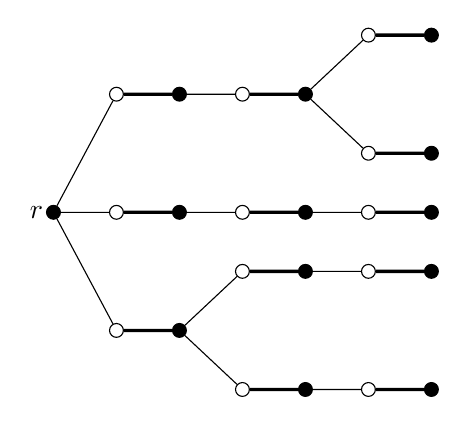
\begin{tikzpicture}
        [
            level distance=8mm,
            every node/.style={draw, fill, circle, minimum size=5pt, inner sep=0pt, line width=0.4pt},
            rootnode/.style={label=left:$r$},
            level 1/.style={nodes={fill=none}, edge from parent/.append style={line width=0.4pt}},
            level 2/.style={nodes={fill}, edge from parent/.append style={line width=1.2pt}},
            level 3/.style={nodes={fill=none}, edge from parent/.append style={line width=0.4pt}},
            level 4/.style={nodes={fill}, edge from parent/.append style={line width=1.2pt}},
            level 5/.style={nodes={fill=none}, edge from parent/.append style={line width=0.4pt}},
            level 6/.style={nodes={fill}, edge from parent/.append style={line width=1.2pt}},
            edge from parent/.style={draw}
        ]

        \node[rootnode] (root) at (0,0) {} [grow = east]
            child {node {} 
                child {node {}
                    child {node {}
                        child {node {} 
                            child {node {}
                                child {node {} 
                                }
                            }
                        }
                    }
                    child {node {}
                        child {node {} 
                            child {node {}
                                child {node {} 
                                }
                            }
                        }
                    }
                }
            } 
            child {node {} 
                child {node {}
                    child {node {} 
                        child {node {}
                            child {node {} 
                                child {node {}}
                            }
                        }
                    }
                }
            }
            child {node {} 
                child {node {}
                    child {node {} 
                        child {node {}
                            child {node {} 
                                child {node {}} 
                            }
                            child {node {} 
                                child {node {}} 
                            }
                        }    
                    }
                }
            };
    \end{tikzpicture}
    \caption{An example of an alternating tree. Nodes in $A_T$ are white while nodes in $B_T$ are black.}
    \label{fig:alternating_tree}
\end{figure}

We can divide an alternating tree $T = (V_T, E_T)$ into two node sets $A_T$ and $B_T$ such that $A_T$ is the set of nodes 
at the other end of an odd-length $M$-alternating path starting at $r$ and $B_T$ is the set of nodes at the other end 
of an even-length $M$-alternating path starting at $r$. Such sets can be built by the following relation: 
starting with $A_T = \emptyset$ and $B_T = \lrc{r}$, if $\lrp{u, v} \in E$ such that $u \in B_T$ and $v \notin A_T \cup B_T$ and there 
exists an edge $\lrp{v, w} \in M$, then $A_T \gets A_T \cup \lrc{v}$ and $B_T \gets B_T \cup \lrc{w}$. 
Note that $\abs{B_T} = \abs{A_T} + 1$. 
Additionally, if there exists some 
edge $\lrp{i, j}$ where $i \in B_T$ and $j \notin T$ such that $j$ is $M$-exposed, then the path $P = \lrp{r, v_1}, \ldots, \lrp{i, j}$
is $M$-augmenting. 

\begin{definition}
    An $M$-alternating tree is \emph{maximal} if for all $b \in B_T$, $\f[N]{b} \sse V_T$ (i.e.\! no additional nodes can be added to the tree).
    It is \emph{frustrated} if for all $b \in B_T$, $\f[N]{b} \sse A_T$.
    \label{def:maximal_alternating_tree}
\end{definition} 

Alternating trees are useful in deciding if a graph has a perfect matching in the following way. 

\begin{lemma}
    Suppose that $G$ has a matching $M$ and an $M$-alternating tree $T$ that is frustrated. Then $G$ has no perfect matching. 
    \label{lem:frustrated_tree_perfect_matching}
\end{lemma}
\begin{proof}
    Consider $G \sm A_T$. The nodes $B_T$ are then single node odd components of $G \sm A_T$ by definition of
    a frustrated tree. Therefore, 
    \begin{equation*}
        \odd{G \sm A_T} \geq \abs{B_T} > \abs{A_T}
    \end{equation*}
    which fails the condition of \cref{thm:tutte_matching}. 
\end{proof}

\subsection{Maximum Cardinality Matchings in the Bipartite Case}

\begin{algorithm}[!h]
    \caption{Maximum Cardinality Matching in Bipartite Graphs} \label{alg:max_card_match_bipartite}
    \begin{algorithmic}[1]
        \Algin A bipartite graph $G = \lrp{V = \lrp{L, R} , E}$
        \Algout A matching $M$ 
        \State $X \gets V, M \gets \emptyset, \calT \gets \emptyset$ \Comment{$X$ is the set of $M$-exposed nodes}
        \While{$X \neq \lrc{\f[\mathrm{root}]{T_i} \colon T_i \in \calT}$} \label{line:max_card_bi_while}
            \State $T \gets \Call{MaximalTree}{G}$%\Call{MaximalTree}{G, X \cap V, M \cap E}$
            \State $\calT \gets \calT \cup T$%, $X \gets X^\prime$, $M \gets M \cup M^\prime$
            \State $G \gets G \sm T$ \Comment{Remove subgraph $T$ from $G$}
        \EndWhile
        \State \Return $M$
        \Statex
        \Function{MaximalTree}{$G = \lrp{V, E}$}
            \State Choose $r \in X \cap V$ \Comment{Choose $M$-exposed vertex in current graph}
            \State $T \gets \lrp{A, B}$ where $A = \emptyset$, $B = \lrc{r}$  
            \While{$\exists e = \lrp{u, v} \in E$ where $u \in B$, $v \notin T$}
                \If{$v \in X$} \Comment{Forms an $M$-augmenting path}
                    \State Let $P$ be the path from $r$ to $v$
                    \State $M \gets \Call{Augment}{M, P}$
                    \State $X \gets X \sm \lrc{r, v}$ 
                    \If{$X = \emptyset$}
                        \State \Return $\emptyset$ %$\lrp{\emptyset, \emptyset, M}$ 
                        \Comment{$M$ is a perfect matching}
                    \Else 
                        \State Choose $r \in X$ \Comment{Start a new $M$-alternating tree}
                        \State $T \gets \lrp{\emptyset, \lrc{r}}$ 
                    \EndIf
                \Else
                    \State $T \gets \Call{ExtendTree}{T, e}$
                \EndIf
            \EndWhile
            \State \Return $T$ %$\lrp{T, X, M}$ 
            \Comment{A maximal $M$-alternating tree is returned}
        \EndFunction
        \Statex
        \Procedure{Augment}{$M$, $P$}
            \State \Return $ M \symdiff P$
        \EndProcedure
        \Statex
        \Procedure{ExtendTree}{$T = \lrp{A, B} , e = \lrp{u, v}$}
            \If{$\exists \lrp{v, w} \in M$}
                \State $A \gets A \cup \lrc{v}$
                \State $B \gets B \cup \lrc{w}$    
            \EndIf
        \EndProcedure
    \end{algorithmic}  
\end{algorithm}

We first note the following. 
\begin{lemma}
    Let $G$ be a bipartite graph. Consider a tree $T$ returned by $\Call{MaximalTree}{G}$. $T$ is maximal. 
    \label{lem:bi_max_card_match_maximal_tree_frustrated}
\end{lemma}
\begin{proof}
    It suffices to show that there exists no edge between any two nodes $b_1, b_2 \in B$. By construction of $T$, if such 
    an edge were to exist, it would form an odd length cycle as any two nodes in $B$ always have an even length path in $T$. 
    However, since $G$ is bipartite, it is impossible for it to have an odd length cycle. Therefore, for all $b \in B$, $\f[N]{b} \sse A$, 
    and $T$ is maximal and frustrated. 
\end{proof}

As an immediate consequence of \cref{lem:frustrated_tree_perfect_matching} and \cref{lem:bi_max_card_match_maximal_tree_frustrated}, 
we get the following. 

\begin{corollary}
    If in the first iteration of \cref{line:max_card_bi_while} a tree $T$ is returned by $\Call{MaximalTree}{G}$, 
    then $G$ has no perfect matching. 
    \label{cor:maximal_tree_bi_no_perf}
\end{corollary}

The correctness of this algorithm is based on the following. 

\begin{theorem}
    Let $G$ be a graph, $M$ a matching on $G$, and $X$ the set of $M$-exposed nodes. Let $\calT$ be a collection of (disjoint) maximal $M$-alternating trees.  
    Define $A = \bigcup_{T_i \in \calT} A_{T_i}$ and $B = \bigcup_{T_i \in \calT} B_{T_i}$. If 
    \begin{itemize}[label=--]
        \item $X = \lrc{\f[\mathrm{root}]{T_i} \colon T_i \in \calT}$
        \item There are no edges between nodes in $B$ 
    \end{itemize}
    then $M$ is a maximum cardinality matching. 
    \label{thm:general_maximal_m_alt_trees_maximum_card}
\end{theorem}
\begin{proof}
    By assumption, there are no edges between nodes in $B$. Additionally, there are no edges 
    between nodes in $B$ and nodes not in $A \cup B$ as they would have been marked as being in $A$
    when creating the $M$-alternating trees. Therefore, all edges with an endpoint in $B$ must have the other endpoint in $A$. 

    By definition of an $M$-alternating tree $T_i$, we have that $\abs{B_{T_i}} - \abs{A_{T_i}} = 1$. Thus, across all trees we have that 
    $\abs{B} - \abs{A} = \abs{\calT}$ (i.e.\! there are $\abs{T}$ $M$-exposed nodes). 
    For a matching to be of greater cardinality than $M$, it must have fewer than $\abs{\calT}$ exposed nodes. 
    However, such a matching still needs to match each node of $B$ onto a node of $A$, so it is not possible for it to have fewer exposed nodes. 
    Therefore, the minimum number of exposed nodes for any matching in $G$ is $\abs{\calT}$, which $M$ achieves. 
\end{proof}

As the above theorem applies to general graphs, we get the following for bipartite graphs.  

\begin{theorem}
    If $G$ is bipartite, the matching $M$ that \cref{alg:max_card_match_bipartite} returns is a maximum cardinality matching. 
    \label{thm:bipartite_max_card_matching}
\end{theorem}
\begin{proof}
    As shown in \cref{lem:bi_max_card_match_maximal_tree_frustrated}, the algorithm must 
    return a collection $\calT$ of maximal $M$-alternating trees such that for each tree $T_i$, there exists no edge between nodes in $B_{T_i}$. 
    Additionally, there do not exist any edges between nodes of $B_{T_i}$ and $B_{T_j}$ for $i \neq j$ as when the first of the two trees 
    were being constructed, such an edge would have been used to extend the tree. 
    Moreover, by design of the algorithm, it must be that $X = \lrc{\f[\mathrm{root}]{T_i} \colon T_i \in \calT}$. 
    Therefore, by \cref{thm:general_maximal_m_alt_trees_maximum_card} $M$ is a maximum cardinality matching. 
\end{proof}

